\section{Satimo StarLab Anechoic Chamber}
The farfield measurements for this project will be carried out in a StarLab anechoic chamber by Satimo. In this section, the principles of doing measurements in this chamber will be described.

\begin{figure}[htbp]
    \centering
    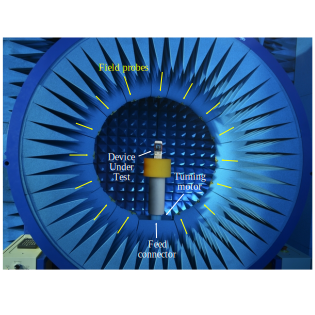
\includegraphics{img/analysis/satimo}
    \caption{Satimo StarLab anechoic chamber. Modified from \cite{satimo}.}
    \label{fig:starlabchamber}
\end{figure}

The Satimo chamber is shown in Figure~\ref{fig:starlabchamber}. It consists of fifteen dual-polarization probes arranged in a circle with \ang{22.5} between each. The probes are located in a circle of absorbing cones and the whole machine is placed in a shielded room.

% Passive measurements: Power -> Antenna -> Probes
% What is measured?
The measurements used in this project are passive measurements. This means that power is supplied from outside the chamber to the Device Under Test (DUT) which then radiates. The source is a user defined frequency sweep. For each frequency, the power at each probe for each polarization is sampled and recorded to a PC. After all frequencies for all probes have been recorded, the bed of the DUT turns, e.g.\ \ang{22.5} and the procedure repeats. The flow is shown in Figure~\ref{fig:satimoflow}.

\begin{figure}[htbp]
    \centering
    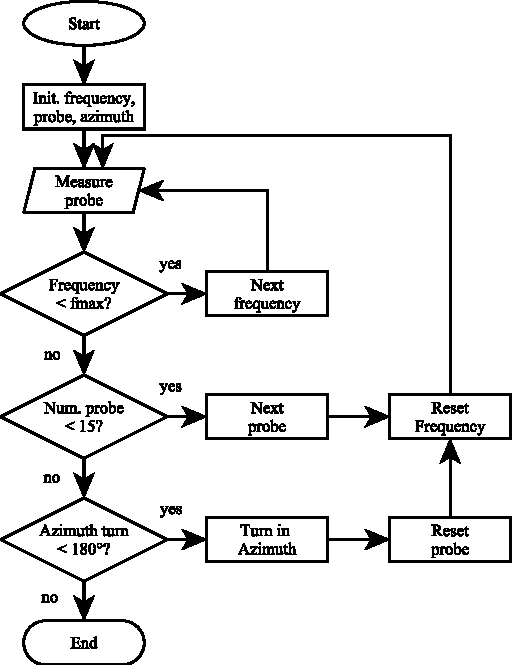
\includegraphics{img/analysis/satimoflow}
    \caption{Flow of a typical passive Satimo measurement.}
    \label{fig:satimoflow}
\end{figure}

% Calibration: Reference gain and efficiency
% What we will use: Efficiency and correlation

